\documentclass[10pt]{article}
\usepackage[T1]{fontenc}\usepackage{lmodern,amsmath,amssymb,graphicx,hyperref}
\usepackage[margin=.75in]{geometry}
\setlength{\parindent}{0pt}\setlength{\parskip}{7pt}
\begin{document}
\begin{center}{\Large Actual pruning and a nonscalar-origin family}\\[4pt]
Local continuation --- 16 November 2026\end{center}
\textbf{Exact pruning.} For the previously constructed integral factorization,
keep label $(r,b)$ precisely when $b+g_q(b)<k$, with $g_q(b)=q$ for odd $b$
and zero for even $b$. Discarded left columns reduce to zero at the actual
creation precision. Applying the shared matrix restriction law preserves
the same reduced polynomial product. No nonzero-support hypothesis is added
[pcc:unverified].

\textbf{Exact cardinalities, not runtime.} Local125/receipt071 gives
\[
|\mathrm{keep}_2|=2^u(k-1)\ (k\ge2),\qquad
|\mathrm{keep}_1|=\begin{cases}2^u(k-1)&k>0\text{ even},\\2^u k&k\text{ odd}.
\end{cases}
\]
Gain zero and $k\le1$ leave the inventory unchanged. These count declared
survivors; they do not establish independence, nonzero rank or a net speedup
[pcc:unverified].

\textbf{A weight collision matters.} Actual rescaled left weight is
$w+b+g_q(b)$. For $q=1$ and $k\ge3$, labels $b=1,2$ both survive and have
weight $w+2$. The declared fiber has exactly $2\cdot2^u$ labels, exceeding
the old $2^u$ bound. Local129/receipt072 proves the collision and a zero/two-bit
alternative: $(r,b)\mapsto(r,b+g_q(b))$ is injective for $q=0,2$ and preserves
weight and side bits. Apply the existing weight-fiber bound to this embedding
[pcc:unverified].

\textbf{Actual policy.} Choose two-bit gain when $i+3\le u$ and zero otherwise.
The existing retained-chart integrality results imply right integrality for
this choice. It preserves the $2^u$ declared capacity but gives up the
available penultimate one-bit gain. This does not reject other one-bit
methods that charge larger fibers [pcc:unverified].

The shifted index is metadata. Its polynomial factor is not proved equal to
the original canonical factor at that shifted index. Original child networks,
entry construction, degree and complete cold bit costs still need bridges.

\textbf{Evidence scope.} Qualifier129 has29 source statements including15
previous count statements. All local statements are outside the shared
Transport53/57 audit and fresh replay. Producer statement/data records are
unsigned and default \texttt{not\_covered} [pcc:unverified].
\newpage
\begin{center}{\Large A degree-preserving change of origin}\end{center}
Let $W$ be the actual completed polynomial matrix and
$D(T)=W_{00}(T)$, independent of the diagonal port. For a public rational
matrix $S$, construct entrywise
\[
 W'(T)=W(T)+D(T)(S-I).
\]
Local131/receipt073 proves seven actual-family statements, including
\[
 W'(0)=S,\qquad W'(t)=W(t)\ (t\ne0\text{ a grid node}),\qquad
 \deg W'_{xy}\le |\mathrm{grid}|-1+\mathrm{mass}.
\]
If $S$ has zero diagonal, the new polynomial diagonal is identically zero.
The degree bound is the old bound, not an assumed favorable cap
[pcc:unverified].

\begin{center}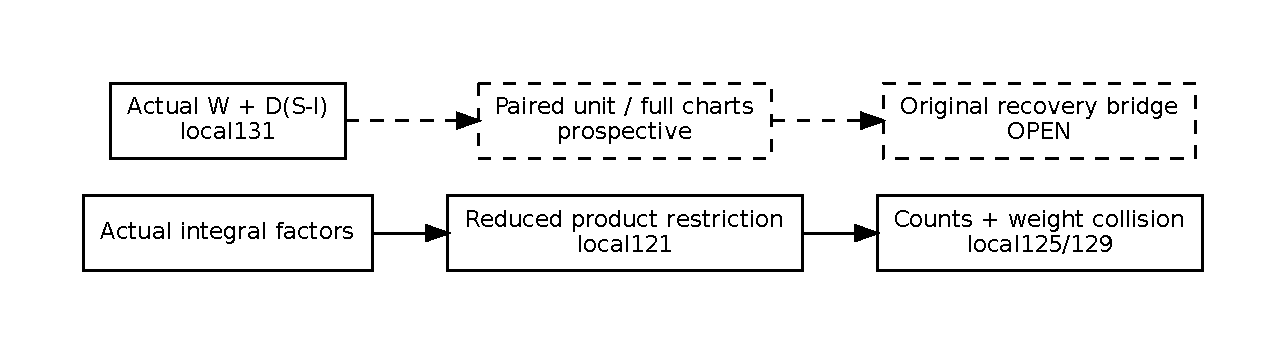
\includegraphics[width=.92\linewidth]{pruning-origin-dependencies-001.pdf}\end{center}

\textbf{Concrete next candidate.} At $a=u+1$, each lower-$u$ residue class has
two ports. Pair them and assign weight
\[
 U_\delta=\prod_{j<u}\left(\frac{2^j}{2^j-\delta}\right)^{m_j},
 \qquad \delta=\pm2^u.
\]
The proposed $S$ is the negative weighted pairing permutation. The target is
an integral inverse and exact partner cancellation, then full retained-node
chart bounds, including anchor zeros. These are prospective obligations at
the scope of this report, not inferred from the seven polynomial statements.

\textbf{Changed premise, explicit test.} This is not $W+C H$: $C(0)=0$,
whereas the new origin is $S$. Preserving nonzero node values alone does not
preserve the original recovery task. Input/output transformation, integral
inverse, weighted modes and recovery equivalence must be proved. The prior
fixed-norm controls show that equal rank does not imply valid relations.

\textbf{Provenance qualifications.} The packaged base121 audit has583
theorems and no extra trusted axioms, but was unpreregistered after a failed
setup; this remains recorded. The older owner receipt's invalid selfbinding
is preserved with a separate correction. No historical byte or claim was
rewritten. No new timing or attack campaign was run [pcc:unverified].
\end{document}
